\subsection{Dati e risultati}

\subsubsection{Generatore di corrente costante.}

Il generatore di corrente costante è stato costruito come nello schema in
figura \ref{fig:generatore1}. La scelta della tensione di input V è stata dettata
dal valore della resistenza R a nostra disposizione e dalla corrente che volevamo
generare: 1 mA. Infatti il polo invertente dell'operazionale è un ground virtuale
(cioè $V_A = 0$), quindi la corrente $I_0$, tenuto conto del fatto che il polo
assorbe una corrente trascurabile, vale $V/R$ (1 mA appunto). 

Poiché abbiamo usato una resistenza R con una tolleranza del 5\%,
che assumo come incertezza sul valore della stessa, e che l'incertezza di risoluzione
sulla tensione V è di 0.005 V, il valore atteso della corrente con l'incertezza è
$I_0 = 1 \pm 0.05$ mA.

Abbiamo misurato con il multimetro la corrente $I_0$ al variare del valore della
resistenza $R_v$, per verificare il funzionamento del generatore. La noiosa
tabella \ref{tab:gen_corr1} mostra che la corrente non varia al variare della resistenza
di carico, proprio come volevamo realizzare. Il circuito si comporta come
una sorgente di corrente costante.

\begin{SCtable}[1][h]
    \centering
    \begin{tabular}{c c}
        \toprule
            $I_0 [\si{\milli\ampere}]$ & $R_v [\si{\kilo\ohm}]$ \\
        \midrule
            $ 1.009 \pm 0.0005 $ & $ 10 $ \\
            $ 1.009 \pm 0.0005 $ & $ 9 $ \\
            $ 1.009 \pm 0.0005 $ & $ 8 $ \\
            $ 1.009 \pm 0.0005 $ & $ 7 $ \\
            $ 1.009 \pm 0.0005 $ & $ 6 $ \\
            $ 1.009 \pm 0.0005 $ & $ 5 $ \\
            $ 1.009 \pm 0.0005 $ & $ 4 $ \\
            $ 1.009 \pm 0.0005 $ & $ 3 $ \\
            $ 1.009 \pm 0.0005 $ & $ 2 $ \\
            $ 1.009 \pm 0.0005 $ & $ 1 $ \\
        \bottomrule
    \end{tabular}
    \caption{La corrente nel circuito \ref{fig:generatore1} rimane costante
        al variare della resistenza di carico $R_v$. Le incertezze riportare sul
        valore di corrente sono incertezze di risoluzione del multimetro
        (metà della risoluzione), mentre sui valori di resistenza non sono riportate
        perchè non rilevanti (sono comunque dell'ordine di qualche ohm).}
    \label{tab:gen_corr1}
\end{SCtable}

\subsubsection{Sommatore pesato di tensioni.}

\begin{SCfigure*}[1][t!]
    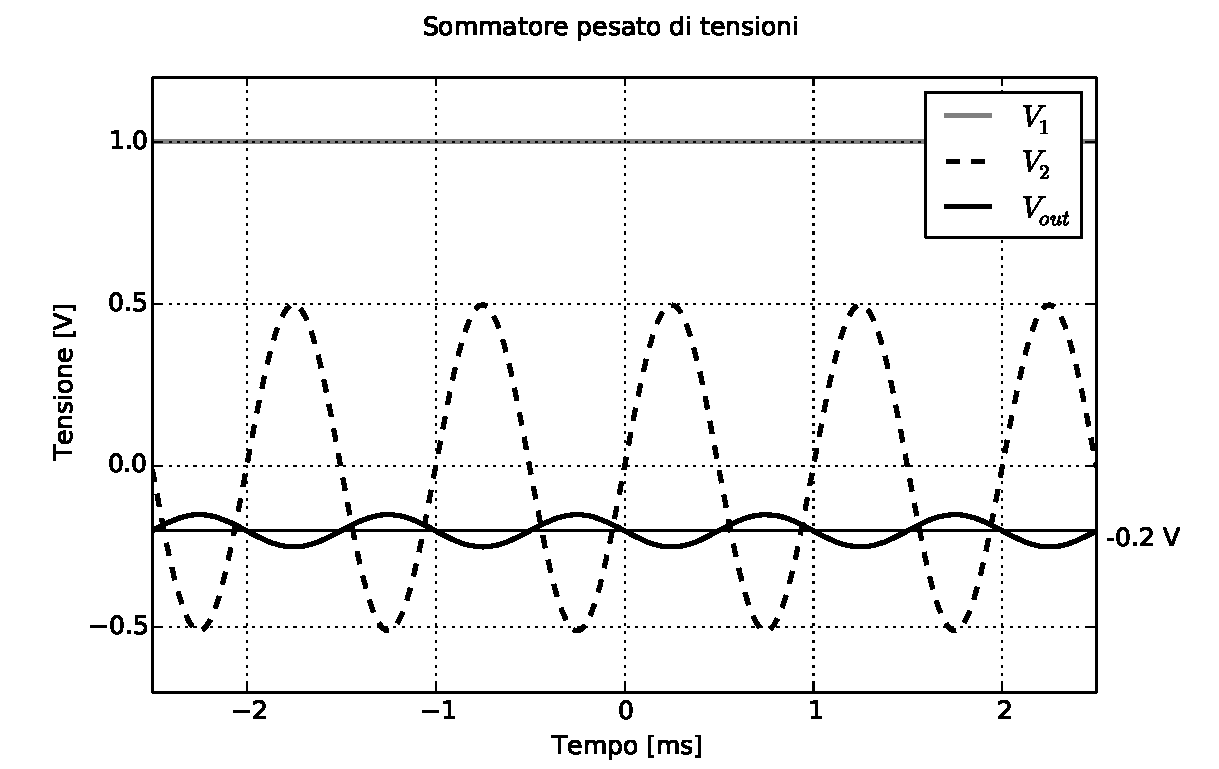
\includegraphics[width=1.4\columnwidth]{figure/graph.pdf}
    \caption{Il grafico riporta un esempio del funzionamento del circuito \ref{fig:sommatore1}.
        I canali $V_1$ e $V_2$ sono stati impostati rispettivamente a una tensione continua di 1 V e
        ad una sinusoide 1 Vpp (peak-to-peak) di frequenza 1 kHz di offset nullo. La sinusoide nera
        mostra l'output: è esattamente quello che ci si aspettava dalla formula \eqref{eq:sommatore_pesato1}.}
    \label{fig:graph1}
\end{SCfigure*}

Il sommatore pesato di tensioni che abbiamo realizzato è il circuito \ref{fig:sommatore1},
ed è pensato per fornire il seguente output

\begin{equation}
    V\ped{out} = R\left(\frac{V_1}{R_1} + \frac{V_2}{R_2}\right)
    \label{eq:sommatore_pesato1}
\end{equation}

Come nel circuito precedente si ha che $V_A = 0$ (ground virtuale) e che
l'amplificatore operazionale assorbe una quantità di corrente trascurabile,
per cui la corrente di retroazione $I_R$ è data dalla somma di $I_1$ e $I_2$
(per la conservazione della carica).
Le resistenze $R_1$ e $R_2$ trasformano le tensioni in ingresso nelle correnti
$I_1$ e $I_2$, pesandole secondo l'inverso dei valori delle stesse.
Questo implica che $I_R$ dipende dalle tensioni in input pesate,
e quindi anche $V\ped{out} = RI_R$ dipende da esse.

La resistenza $R$ determina il guadagno del circuito. Per esempio per la tensione
$V_1$ il guadagno vale

\begin{equation}
    G = \frac{V\ped{out}}{V_1} = \frac{R}{R_1} = 0.2 \pm 0.014
\end{equation}

dove abbaimo considerato incertezze sulle resistenze pari al 5\%.

Per verificare il corretto funzionamento del circuito abbiamo generato due segnali,
usando il generatore di forme d'onda a nostra disposizione e quello integrato
nell'oscilloscopio, e li abbiamo dati in input al circuito. Poi con l'oscilloscopio
abbiamo verificato che l'output si comportasse secondo la \eqref{eq:sommatore_pesato1}.
Il risultato è stato positivo: abbiamo provato diverse combinazioni di sinusoidi,
onde quadre, rampe e triangoli e in tutti i casi il circuito si è comportato correttamente.

Purtroppo l'oscilloscopio a nostra disposizione non ha 3 canali in ingresso (che sarebbero
stati utili per vedere contemporaneamente i due input e l'output), per cui abbiamo dovuto
usare la funzione di persistenza per visualizzare i 3 segnali, che non permette di salvare i dati.
A causa di questo fatto non siamo riusciti a riportare i grafici che mostrino il funzionamento
del circuito.

Siamo quindi tornati in laboratorio alcuni giorni dopo e abbiamo montato il circuito una seconda
volta per acquisire almeno un grafico che mostrasse il funzionamento del circuito.
Il risultato è riportato in figura \ref{fig:graph1}. Per motivi di chiarezza del grafico, abbiamo
scelto $V_1 = 1$ V DC, mentre $V_2$ era un onda sinusoidale di frequenza 1 kHz e di ampiezza 1 V
picco-picco. L'output è riportato in figura e corrisponde a quanto previsto dalla
formula \eqref{eq:sommatore_pesato1}.

Il guadagno per $V_1$ è esattamente 0.2 come calcolato sopra. L'amplificatore è invertente.